\hypertarget{what-exactly-is-a-robot}{%
\section{What exactly is a robot?}\label{what-exactly-is-a-robot}}

\begin{figure}
\centering
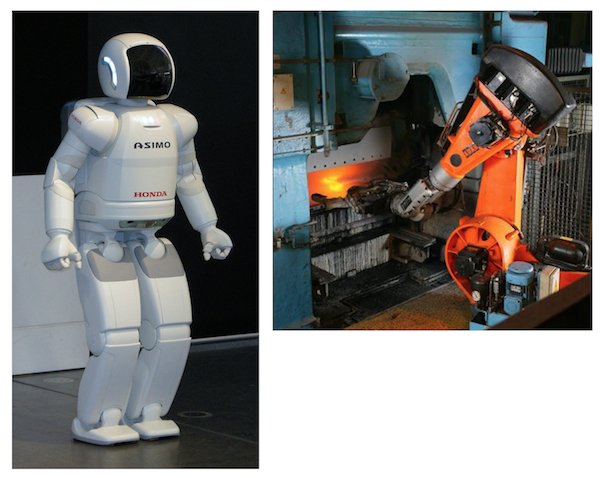
\includegraphics[width=0.9\textwidth,height=\textheight]{IntroductionFigures/honda-foundry.*}
\caption{Two different versions of robots. a) \texttt{Honda\ Asimo}
Robot \texttt{Asimo} b) \texttt{Kuka\ robot} \texttt{Kuka}}
\end{figure}

\hypertarget{definition}{%
\subsection{Definition}\label{definition}}

What is a \texttt{robot}? This is actually a complicated question.
Wikipedia defines a robot in the following manner: \emph{A robot is a
mechanical intelligent agent which can perform tasks on its own, or with
guidance; usually an electro-mechanical machine which is guided by
computer and electronic programming.} (There are plenty of opinions on
Wikipedia. I find that it is pretty good for math, science and
engineering quick reference but not always an expository presentation.
It is also good at reflecting opinions, which in this case is useful.)
Merriam-Webster, on the other hand, says a robot is \emph{a real or
imaginary machine that is controlled by a computer and is often made to
look like a human or animal.} According to the Encyclopaedia Britannica,
a robot is \emph{any automatically operated machine that replaces human
effort, though it may not resemble human beings in appearance or perform
functions in a humanlike manner}.

This latter definition includes washing machines, bread makers, and
other devices not generally seen as a robot. However, as we will argue,
that does not matter! A definition of robot that uses form or motion is
flawed. What if we made the statement broader? \textbf{A robot is seen
as a sophisticated machine that, as stated above, replaces human
effort}. Nothing else really defines robotics as well.

Regardless of definition, these machines surround us. Today we can see
them used from manufacturing to exploration, from assistive technologies
and medicine to entertainment, from research to education, and much
more.

\begin{figure}
\centering
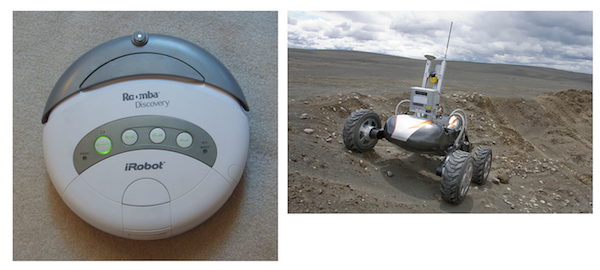
\includegraphics[width=0.9\textwidth,height=\textheight]{IntroductionFigures/roomba-drill.*}
\caption{More examples of assistive robots. a) iRobot \texttt{Roomba}
Discovery 2.1. \texttt{Roomba} b) NASA experimental drilling robot.
\texttt{DrillingRover}}
\end{figure}

There is no consensus on which machines qualify as robots. However,
there \emph{is} a general agreement that robots exhibit behaviors which
mimic humans or animals - that is, \emph{behavior which seems
intelligent.} We expect the robot to interact with its environment and
the objects within that environment. Most of us may expect that the
robot performs this interaction through movement and sensation.

\begin{figure}
\centering
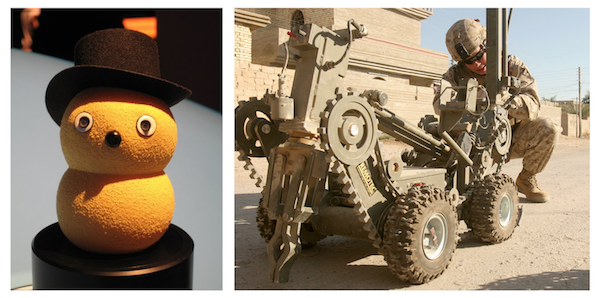
\includegraphics[width=0.9\textwidth,height=\textheight]{IntroductionFigures/keepon-ied.*}
\caption{There are a wide range of roles for robots. a) \texttt{Keepon}
- therapy robot. \texttt{Keepon} b) Robot tasked to detonate a buried
improvised explosive device. \texttt{IEDbot}}
\end{figure}

Many may expect the robot to perform complex tasks or deal with harsh,
unforgiving environments. Some may expect a robot to be an extension of
themselves through teleoperation or remote control, while others expect
it to be a fully autonomous device.

We can boil down our notion of robot abilities to three things:

\begin{description}
\item[\textbf{Perception:}]
sensing the environment and to a limited degree understanding the
sensory information.
\item[\textbf{Cognition:}]
ability to make decisions and responses based on the sensory information
and not acting in a pre-programmed manner.
\item[\textbf{Actuation:}]
full mobility of the machine or control of a tool through a manipulator.
\end{description}

\begin{figure}
\centering
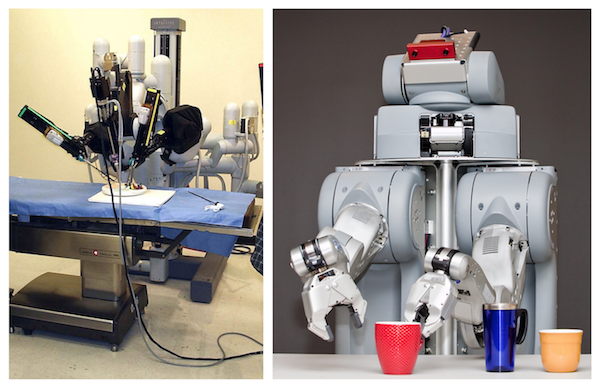
\includegraphics[width=0.9\textwidth,height=\textheight]{IntroductionFigures/davinci-pr2.*}
\caption{Systems which focus on manipulation: a) \texttt{Da\ Vinci}
Surgical System \texttt{DaVinci} . b) Willow Garage's \texttt{PR2}
robot. \texttt{WGPR2}}
\end{figure}

One interesting phenomenon that could be influencing the lack of a solid
definition for the term is that what we label a ``robot" varies with
time. When a new capability arises, one that was previously considered
to be solely in the domain of humans and animals, we tend to label it a
robot. As soon as that capability becomes routine, the device is thought
of a mechatronic device.

\begin{figure}
\centering
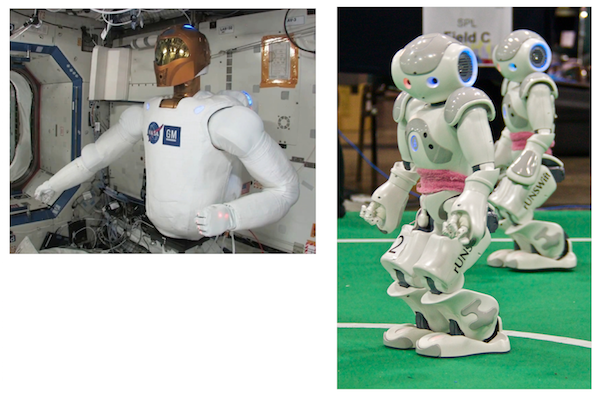
\includegraphics[width=0.9\textwidth,height=\textheight]{IntroductionFigures/nasa-nao.png}
\caption{Systems which focus on mobility: a) NASA's \texttt{Robonaut}.
\texttt{Robonaut} b) \texttt{RoboCup} Standard Platform League (Image
from 2010). \texttt{Robocup}}
\end{figure}

Robots embody technological magic. So, it is natural that some
previously unseen ability programmed into a machine will have a magic
quality for humans, thus making that machine more of a robot. But with
time, we get accustomed to it, and the magic gets replaced with
expectation.

\begin{figure}
\centering
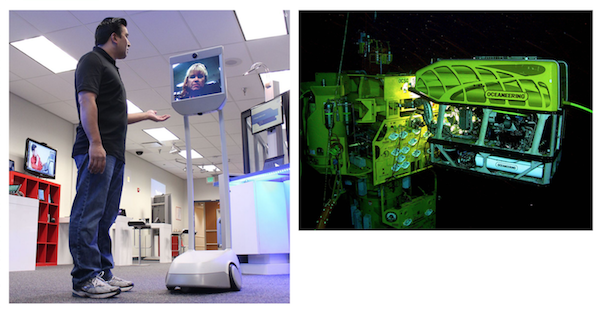
\includegraphics[width=0.9\textwidth,height=\textheight]{IntroductionFigures/beam-rov.*}
\caption{Telepresence or remote work is a growth area in robotics. a) An
Intel IT Labs researcher working on a remote telepresence robot pilot
project that uses Suitable Technologies' Beam robot. \texttt{TelePR} b)
ROV working on a subsea structure. \texttt{ROV}}
\end{figure}

It can be argued that there is nothing new in the subject of robotics
-that all we are doing is building machines. Nothing different than what
engineers have been doing all along. The term robotics has more to do
with our ego and psychology than anything to do with science and
technology. However, there is a body of knowledge related to building
machines that interact in human or physical environments. This is what
we will consider robotics.

\begin{figure}
\centering
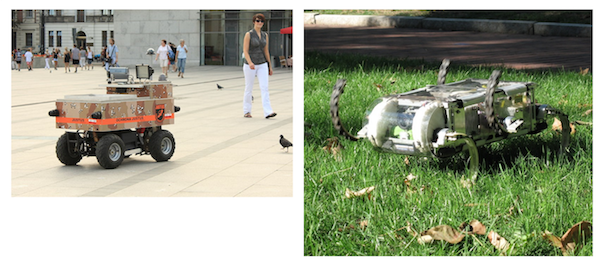
\includegraphics[width=0.9\textwidth,height=\textheight]{IntroductionFigures/justus-rhex.*}
\caption{Mobility in simple and complex domains. a) Justus security
robot in front of Krakow railway station \texttt{Justus}. b) Rhex: DARPA
project on compliant six legged robots. \texttt{RHex}}
\end{figure}

\hypertarget{a-brief-history}{%
\subsection{A brief history}\label{a-brief-history}}

\hypertarget{bc}{%
\subsubsection{1023 BC}\label{bc}}

In ancient China, a curious account on automata is found in the Lie Zi
text, written in the 3rd century BC. Within it there is a description of
an encounter between King Mu of Zhou (1023-957 BC) and a mechanical
engineer known as Yan Shi, who was an 'artificer'. According to the
text, the \texttt{artificer} proudly presented the king with a
life-size, human-shaped figure of mechanical handiwork which could sing
and move in a life-like manner.

\hypertarget{bc-1}{%
\subsubsection{205 BC}\label{bc-1}}

In ancient Greece, an orrery known as the \texttt{Antikythera} Mechanism
is developed. This device is credited as being the first analog
computer.

\begin{figure}
\centering
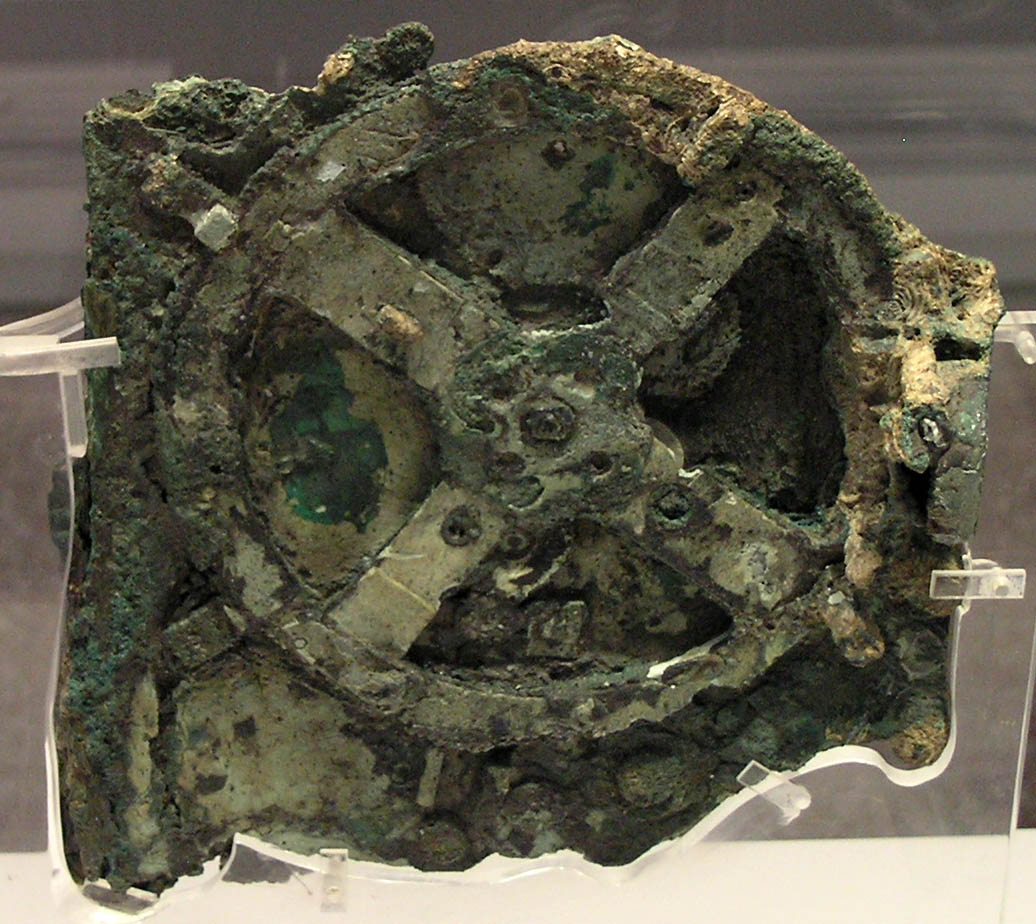
\includegraphics[width=0.4\textwidth,height=\textheight]{IntroductionFigures/antikytheramachine.*}
\caption{Antikythera Mechanism \texttt{Antikythera}.}
\end{figure}

\hypertarget{bc-2}{%
\subsubsection{270 BC}\label{bc-2}}

The Greek engineer \texttt{Ctesibius} (c. 270 BC) applies a knowledge of
pneumatics and hydraulics to produce the first organ and water clocks
with moving figures.

\hypertarget{ad}{%
\subsubsection{1088 AD}\label{ad}}

The Cosmic Engine, a 10-meter (33 ft) clock tower built by Su Song in
Kaifeng, China. It featured mechanical mannequins that chimed the hours,
ringing gongs or bells among other devices.

\hypertarget{ad-1}{%
\subsubsection{1206 AD}\label{ad-1}}

\texttt{Al-Jazari} (1136-1206), an Arab Muslim inventor during the
Artuqid dynasty, designed and constructed a number of automatic
machines, including kitchen appliances, musical automata powered by
water, and the first programmable humanoid robot in 1206. Al-Jazari's
robot was a boat with four automatic musicians that floated on a lake to
entertain guests at royal drinking parties. His mechanism had a
programmable drum machine with pegs (cams) that bump into little levers
that operate the percussion. The drummer could be made to play different
rhythms and different drum patterns by moving the pegs to different
locations.

\begin{figure}
\centering
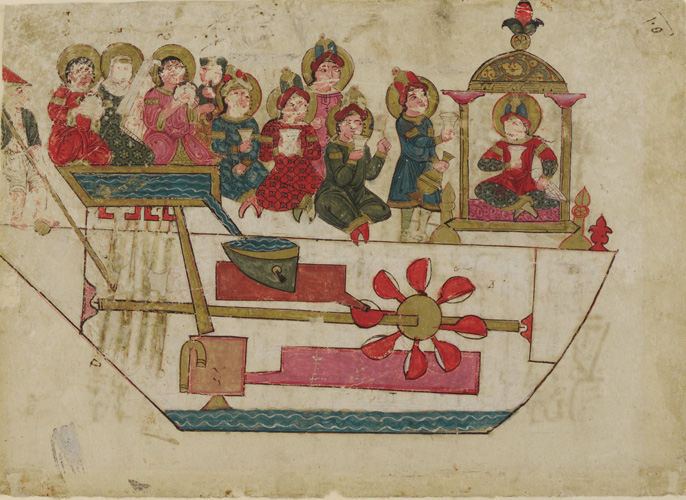
\includegraphics[width=0.4\textwidth,height=\textheight]{IntroductionFigures/Al-Jazari.*}
\caption{Al-Jazari's Mechanical Musical Boat. \texttt{AlJazari}.}
\end{figure}

\hypertarget{section}{%
\subsubsection{1495}\label{section}}

Leonardo da Vinci draws plans for a mechanical knight.

\hypertarget{section-1}{%
\subsubsection{1922}\label{section-1}}

The word \emph{robot} is introduced to the English language through the
play \texttt{Rossum’s\ Universal\ Robots} by the Czech writer Karel
\texttt{Capek}. The play is centered around a factory staffed by
intelligent cyborgs. The English term robot comes from the Slavic word
\emph{robota} which roughly translates as work or labor. Credit for the
term goes to Karel's brother Josef.

\hypertarget{section-2}{%
\subsubsection{1954}\label{section-2}}

Following World War II, efforts in automation increased. Early advances
were seen in teleoperation and computer numerically controlled (CNC)
machining. General Electric produced machines that had a master slave
approach where the master manipulator would control the slave. The CNC
machines gained popularity in the aircraft industry by milling high
performance parts in lower volumes. The merger of these two technologies
produced the first programmed articulated device by George Devol in
1954. He replaced the master manipulator with CNC technology. Joseph
Engelberger purchased the rights and founded Unimation in 1956.
Unimation placed its first robot arm in a General Motors plant in 1961.

\hypertarget{section-3}{%
\subsubsection{1969}\label{section-3}}

The 1960's saw significant experimentation with manipulator designs,
feedback systems and actuator types. One such example of a robotic
manipulator is the Stanford Hydraulic Arm and Stanford Manipulator,
designed in 1969 by Victor Scheinman, a Mechanical Engineering student
working in the Stanford Artificial Intelligence Lab (SAIL).

\hypertarget{section-4}{%
\subsubsection{1973}\label{section-4}}

The Cincinnati Milacron \(T^3\) is released. It was a heavy lift
assembly line manipulator. In 1978, Unimation introduced the PUMA,
(Programmable Universal Machine for Assembly) and JPL started a research
program to develop space based teleoperated manipulators. By the late
1970's, applications for industrial robots grew quickly and robots in
industry became established.

The history for mobile robots is much more recent. The challenges for
mobile robots, as we will see later on, are fundamentally different than
industrial automation. An early example is the Johns Hopkins
\emph{Beast}. It was a simple autonomous mobile system that navigated
using touch sensors and could recharge itself. This system required an
instrumented environment. A notable development is \emph{Shakey}, by the
Stanford Research Institute (SRI) from 1966-72. This robot implemented
computer vision and natural language processing and is responsible for
the development of the A* search algorithm, the Hough transform, and
visibility graphs.
